\documentclass{beamer}
\usepackage{beamerthemeshadow}
\usepackage{graphicx}
\usepackage{color}
\usepackage[T1]{fontenc}
\usepackage[utf8]{inputenc}
\usepackage{hyperref}
\usepackage[flushleft]{threeparttable}
\usepackage{multicol} %da bi napisalo formule za amdalov zakon jedna do druge
\usepackage[english, serbian]{babel}
\usepackage{makecell}
\usepackage{listings}

\definecolor{beamer@boja}{rgb}{0.5,0.1,0.5}
\setbeamercolor{structure}{fg=beamer@boja}

\def\d{{\fontencoding{T1}\selectfont\dj}}
\def\D{{\fontencoding{T1}\selectfont\DJ}}


\title{Paralelno programiranje}
\subtitle{-- Seminarski rad --}
\author{Aleksandar Đukić, Marija Zrnić, Iva Minić, Luka Mitrović}
\institute{Matematički fakultet\\Univerzitet u Beogradu}
\date{
	\footnotesize{Beograd, 2022.}	
}

\begin{document}
	\begin{frame}
		\thispagestyle{empty}
		\titlepage
	\end{frame}
	
	\addtocounter{framenumber}{-1}
	
	\begin{frame}[fragile]\frametitle{Literatura}
		\begin{itemize}
			\item Zasnovano na:\\
			Aleksandar Đukić, Marija Zrnić, Iva Minić, Luka Mitrović: Paralelno programiranje, 2022.\\
			\emph(\url{https://github.com/mi22092/7_TNP2022/blob/main/7_%C4%90uki%C4%87Zrni%C4%87Mini%C4%87Mitrovi%C4%87/7_%C4%90uki%C4%87Zrni%C4%87Mini%C4%87Mitrovi%C4%87.pdf})
			%Goran Nenadic, Predrag Janičić, Aleksandar Samardžić: \LaTeX{} za autore, Beograd, Kompjuter biblioteka, 2003.
			%(\url{http://poincare.matf.bg.ac.rs/~janicic//latex2e/})
		\end{itemize}
	\end{frame}
	
	\begin{frame}
		\frametitle{Pregled}
		\tableofcontents[hidesubsections] 
	\end{frame}
	
	\section{Uvod i istorija}
	
	\begin{frame}[fragile]\frametitle{Uvod i istorija}
		\begin{itemize}	
			\item Pojam paralelnog programiranja
			\item Razlika između paralelne obrade i paralelnog programiranja
			\bigskip
			\item Paralelna obrada se prvi put pominje 1950-ih
			\item 1962. Burroughs proizvodi sistem D825 sa 4 procesora
			\item 1967. Amdalov zakon nastaje na \emph{Spring Joint} konferenciji
			\item 1983. \emph{Caltech} proizvodi \emph{The Cosmic Cube} sa 64 procesora
			\bigskip
			\item 1992. \emph{Standards for Message-Passing in a Distributed Memory Environment} radionica; 1994. \emph{MPI} interfejs
			\item 1997. \emph{OpenMP Architecture Review Board} objavljuje interfejs \emph{OpenMP} za \emph{Fortran}, zatim za C/C++.
		\end{itemize}
	\end{frame}
	
	
	%\subsection{Princip rada}
	\section{Princip rada paralelnog programiranja}
	\subsection{Osnove i forme paralelne obrade}
	\begin{frame}[fragile]\frametitle{Osnove i forme paralelne obrade}
		\begin{itemize}	
			\item Forme paralelne obrade:
			\begin{itemize}
				\item \textbf{Nivo bita} (eng. \emph{bit-level})
				\item \textbf{Nivo naredbe} (eng. \emph{instruction level})
				\item \textbf{Paralelizam podataka} (eng. \emph{data parallelism})
				\item \textbf{Paralelizam zadataka} (eng. \emph{task parallelism})
			\end{itemize}
			%ovde moze da ide ona tabela sa formama samo skraceno
		\end{itemize}
		\begin{table}[h]
			\begin{center}
			\resizebox{8cm}{!}{
			\renewcommand{\arraystretch}{2}
				\begin{tabular}{ |c|c| }
					\hline
					Naziv & Formula \\
					\hline 
					\makecell{Amdalov zakon} & $S_{max} = \frac{1}{(1 - p) + \frac{p}{s}}$ \\[8pt] 
					\hline 
					\makecell{Gustafsonov zakon} & $S_{max} = N + (1 - N) * s$ \\
					\hline
				\end{tabular} }
				\caption{Modeli izračunavanja efikasnosti paralelne obrade}
			\end{center}
		\end{table}
	\end{frame}

	\subsection{Koraci paralelizacije i modeli paralelnog programiranja}
	\begin{frame}[fragile]\frametitle{Koraci paralelizacije i modeli paralelnog programiranja}
	\begin{itemize}	
		\item Koraci paralelizacije programa:
		\begin{itemize}	
			\item \textbf{Dekompozicija} - Razdvaja obradu na više zadataka
			\item \textbf{Dodela} - Zadaci se dele među procesima, \textbf{\emph{particionisanje}}
			\item \textbf{Orkestracija} - Organizuje rad
			\item \textbf{Mapiranje} - Deli procese među procesorima  
		\end{itemize} 
		\bigskip
		\item \textbf{Komunikacija} - Razmena podataka između procesa koji se trenutno izvršavaju
		\bigskip
	 		\item Modeli paralelnog programiranja:
				\begin{itemize}	
					\item \textbf{Model deljene memorije} (eng. \emph{shared memory model})
					\item \textbf{Model prenošenja poruke} (eng. \emph{message passing model})
					\item \textbf{Particionisani globalni adresni prostor} (eng. \emph{partitioned global address space}) -- hibridni model
				\end{itemize}
	\end{itemize}
	\end{frame}
	% predlog - ispod koraka staviti modele i izbaciti sledeci slajd (tesno je ali moze da stane)
	
	\section{Upotrebe, prednosti i mane}
	\begin{frame}[fragile]\frametitle{Upotrebe, prednosti i mane}
		\begin{itemize}	
			\item Paralelno programiranje koristimo kada imamo velike količine podataka, kompleksne račune ili velike simulacije.
			\item Neke od oblasti u kojima se paralelno programiranje koristi su primenjena fizika, elektrotehnika, finansijsko i ekonomsko modeliranje, veštačka inteligencija, kvantna mehanika i druge.
			\bigskip
			\item Prednosti paralelnog programiranja: brzina, poboljšan GUI (\emph{grafički korisnički interfejs}), istovremeno pokretanje različitih logika programiranja, bolje korišćenje keš memorije i CPU resursa.
			\item Mane paralelnog programiranja: promena konteksta, nepredvidljivost, otežano programiranje, \emph{data race} i \emph{deadlock}.
		\end{itemize}
	\end{frame}
	
	\section{Primer}
    \begin{frame}[fragile]\frametitle{Primer - Prebrojavanje prostih brojeva u listi}
        \begin{itemize}
            \item Modul \emph{multiprocessing}, klasa \emph{Pool}
        \end{itemize}
    \begin{lstlisting}[showstringspaces=false, language=Python]
pool = multiprocessing.Pool(processes=4)
nums_list = generate_list(15000, 9, 12)
nums_list = chunks(nums_list, 4)
print(sum(pool.map(count_primes, nums_list)))
    \end{lstlisting} 
    \begin{figure}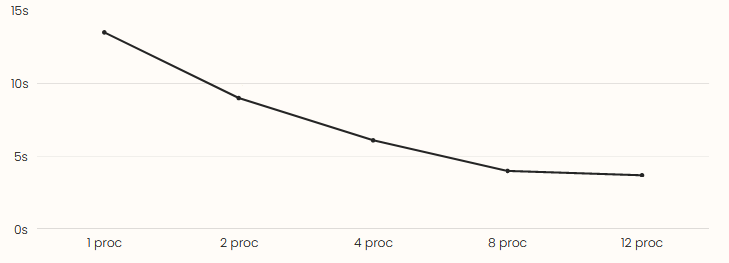
\includegraphics[height=3cm]{grafik_prez.png}
    \caption{Performanse}
    \end{figure}
    \end{frame}
    \section{Zaključak}
    \begin{frame}[fragile]\frametitle{Zaključak}
        \begin{itemize}
            \item Pogodna tehnika za ubrzanje određenih vrsta programa
            \item Sjajna budućnost, velikim delom zbog fizičke ograničenosti modernih mikroprocesora
        \end{itemize}
    \end{frame}
	%primeri
	

	%\section{Zakljucak}
	%\begin{frame}[fragile]\frametitle{Zaključak}
		%zakljucak
	%\end{frame}
	
\end{document}
